\documentclass[journal]{new-aiaa}
%\documentclass[conf]{new-aiaa} for conference papers
\usepackage[utf8]{inputenc}
\usepackage{textcomp}

\usepackage{graphicx}
\usepackage{amsmath}
\usepackage[version=4]{mhchem}
\usepackage{siunitx}
\usepackage{longtable,tabularx}
\usepackage{mylistingstyle}
\usepackage{longtable}
\setlength\LTleft{0pt} 

\title{Streamlined Image Preprocessing Framework for Computer Vision Applications %\\[10pt]
%\normalsize\textit{\today}  % Smaller font size and italics for the date
}

\author{Author: Luis Kraker\footnote{BsC, Master's student in System Test Engineering, FH-Joanneum}}
\affil{FH-Joanneum, Graz 8020, Austria}
\author{Supervisor: Mrs. Gudrun Schappacher Tilp\footnote{DDr, Associate Professor at FH-Joanneum}}
\affil{FH-Joanneum, Graz 8020, Austria}

\begin{document}

\maketitle
% \begin{center}
% 	\today
% \end{center}

\begin{abstract}
This paper introduces a modular image preprocessing framework designed to streamline the setup and application of preprocessing pipelines in computer vision tasks. Leveraging the robust functionalities of TensorFlow and OpenCV, our framework offers a user-friendly interface that simplifies experimentation and enhances reproducibility. We detail the framework's architecture, which supports easy integration and extension with new preprocessing techniques, and demonstrate its application with a simple example. By simplifying the preprocessing process, our framework not only improves the efficiency of data preparation but also allows practitioners to focus more on model innovation and less on routine data manipulation.
\end{abstract}


\section{Introduction}
\lettrine{T}{he} field of computer vision is increasingly prevalent, significantly impacting both industry and daily life. It enhances consumer multimedia experiences, operates household robotics, streamlines manufacturing processes, aids in medical diagnostics and treatments, and powers autonomous vehicles.\cite{bebis2002review} Beyond these applications, computer vision continues to expand into new areas, further integrating into our everyday experiences.\cite{szeliski2010computer}


Central to these applications is image preprocessing, which prepares images for subsequent analysis and feature extraction.\cite{gonzalez2002digital} Effective image preprocessing improves image quality, facilitates the extraction of relevant features, and accelerates the entire machine learning pipeline driving computer vision applications.\cite{nelson2020image}\cite{krig2014image}

Despite the importance of image preprocessing, using popular libraries like TensorFlow (\cite{tensorflow2015}) and OpenCV (\cite{opencv2000}) without high-level abstraction often presents challenges:
\begin{itemize}
	\item Experimentation with different techniques or parameters is difficult due to scattered code.
	\item Reproducibility is hindered by the lack of straightforward methods to save and load preprocessing pipelines.
	\item Lack of modularity makes the code tightly coupled with the rest of the codebase, complicating maintenance and updates.
	\item Integrating preprocessing routines with various machine learning frameworks often requires duplicating code.
	\item The complexity of existing solutions can be frustrating for beginners.
\end{itemize}

To overcome these challenges, we propose a simple, modular image preprocessing framework that offers a streamlined interface for common preprocessing tasks.  Built on OpenCV and TensorFlow, this framework provides a beginner-friendly Application Programming Interface (API) that facilitates experimentation, ensures reproducibility through easy pipeline management, allows for automatic experimentation and improves modularity for better integration with diverse machine learning environments. Leveraging Python as the programming language it guarantees broad accessibility and seamless integration with existing projects.\cite{python}\cite{pythonCV} This paper details the design and implementation of our framework and includes a practical demonstration of its capabilities.


\section{Implementation}
The image preprocessing framework developed benefits from the capabilities of TensorFlow and OpenCV. TensorFlow, a robust machine learning library, provides extensive end-to-end machine learning tools optimizing computational efficiency and allowing for the integration of complex machine learning functionalities.\cite{tensorflowLearn} OpenCV is used for its advanced image processing capabilities, offering a range of operations that are not available in TensorFlow, thus enriching the framework's processing abilities.\cite{opencvTutorial}


\subsection{Framework Overview}
Inspired by the scikit-learn's Pipeline design, our framework enables chaining multiple image processing steps into a structured pipeline, specifically designed for image data.\cite{pedregosa2011scikit} Unlike scikit-learn, which is generally used for tabular data, our framework focuses exclusively on image preprocessing without extending into model training.

The primary objective of the framework is to simplify and streamline the image preprocessing pipeline for computer vision tasks. Specifically, it aims to:
\begin{itemize}
	\item Enable easy chaining of multiple image processing steps.
	\item Facilitate the application of these steps to complete datasets efficiently.
	\item Allow for straightforward randomization of pipeline configurations, beneficial for hyperparameter optimization.
	\item Provide simple mechanisms for saving and loading pipelines, enhancing reproducibility and ease of experimentation.
	\item Ensure the framework is easily extendable with new image processing steps, meeting changing requirements and new techniques.
\end{itemize}

\subsection{Framework Architecture}
\label{sec:framework_architecture}
Our framework uses a carefully chosen architecture that promotes straightforwardness, efficiency and modularity. To achieve these goals, the framework is built around several core components, each fulfilling a unique role in the pipeline. The primary components of the framework are as follows:

\begin{itemize}
	\item \texttt{ImagePreprocessor} class serves as the central component of the framework. It manages the configuration and execution of the image preprocessing pipeline.
	\item \texttt{StepBase} class acts as an abstract base class for all preprocessing steps, ensuring consistency and providing common functionalities.
	\item \texttt{ClassInstancesSerializer} class provides methods for serializing and deserializing the pipeline configurations, facilitating reproducibility and experimentation.
	\item \texttt{Preprocessing Steps} encapsulate specific preprocessing operations within subclasses of \texttt{StepBase}, enhancing the framework's modularity.
\end{itemize}

% The simplified Unified Modeling Language (UML) diagram in Figure~\ref{fig:framework_uml} illustrates the relationships between these classes and their public methods.

% \begin{figure}[h]
% 	\centering
% 	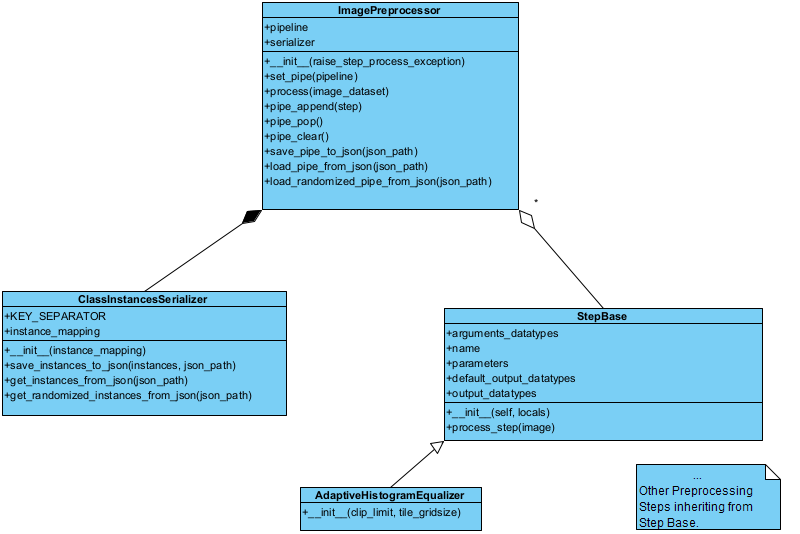
\includegraphics[width=0.8\textwidth]{image_preprocessing_uml.png}
% 	\caption{Simplified UML Diagram of the Image Preprocessing Framework}
% 	\label{fig:framework_uml}
% \end{figure}

% \newpage

\subsection{Preprocessing Operations}
Each preprocessing operation is encapsulated within a subclass of \texttt{StepBase}, implementing specific functionalities such as adaptive histogram equalization. These classes highlight the framework's modularity, allowing users to easily customize and extend the pipeline. Listing ~\ref{lst:preprocessing_step} demonstrates the implementation of an adaptive histogram equalization step, that can be seamlessly integrated into the preprocessing pipeline. The example shows the simplicity of adding new preprocessing steps to the framework.\\

\begin{lstlisting}[language=Python, caption=Example of a Preprocessing Step Implementation, label=lst:preprocessing_step]
class AdaptiveHistogramEqualizer(StepBase):
    arguments_datatype = {'clip_limit': float, 'tile_gridsize': (int, int)}
    name = 'Adaptive Histogram Equalizer'

    def __init__(self, clip_limit=2.0, tile_gridsize=(8,8)):
        super().__init__(locals())

    @StepBase._nparray_pyfunc_wrapper
    def process_step(self, image_nparray):
        channels = cv2.split(image_nparray)
        clahe = cv2.createCLAHE(clipLimit=self.parameters['clip_limit'],
                                tileGridSize=self.parameters['tile_gridsize'])
        clahe_channels = [clahe.apply(ch) for ch in channels]
        clahe_image = cv2.merge(clahe_channels)
        return clahe_image
\end{lstlisting}

\subsection{Serialization and Deserialization}
The framework offers a direct method for serializing and deserializing the preprocessing pipeline configuration, enabled by  the \texttt{ClassInstancesSerializer} class. This class handles the conversion of the pipeline configuration into a JSON format and back, taking advantage of JSON's readability, editability, and hierarchical organization, which suits the pipeline's structure. The \texttt{ClassInstancesSerializer} also manages the datatypes of the pipeline parameters to ensure they are compatible with JSON formatting. It is responsible for converting the parameters of the preprocessing steps into a format that can be serialized in JSON and for restoring the original datatypes upon deserialization. To serialize new preprocessing steps, simply define the parameter datatypes in the \texttt{arguments\_datatype} class variable, and the \texttt{ImagePreprocessor} in conjunction with the \texttt{ClassInstancesSerializer} will handle the serialization and deserialization accordingly.


\subsection{Testing Strategies of the Framework}
The reliability of our framework is supported by a detailed testing strategy that uses Python's \texttt{unittest} module.\cite{unittestPython} Each main class within the framework, as detailed in section \ref{sec:framework_architecture}, has its own set of tests. These include unit tests, which verify the functionality of individual methods, and integration tests, which evaluate how well the classes work together.

To ensure uniformity across the preprocessing steps and minimize redundant testing efforts, we have established a common test suite. This suite is designed to check the correctness of the preprocessing steps and their integration within the framework. It is consistently used across all preprocessing components to maintain standards and prevent errors.

Additionally, we provide a thorough testing scenario called the "long pipeline test." This test is essential for assessing the framework’s ability to handle long preprocessing pipelines. It involves testing several extended pipelines, each containing numerous preprocessing steps, on various images. The order of the steps in these pipelines is varied to ensure the framework can manage different configurations effectively. This test is crucial for verifying that complex preprocessing pipelines are executed efficiently and accurately by the framework.


\section{Application}
Given the detailed implementation described, the image preprocessing framework provides a user-friendly and intuitive process for setting up and applying image preprocessing pipelines.

\subsection{Setting Up the Preprocessing Pipeline}
The steps to configure the preprocessing pipeline are outlined below:

\begin{enumerate}
	\item Instantiate the \texttt{ImagePreprocessor} class.
	\item Construct the preprocessing pipeline by specifying the sequence of desired preprocessing steps.
	\item Set the configured pipeline to the \texttt{ImagePreprocessor} instance.
	\item Finally, apply the pipeline to the image dataset for processing.
\end{enumerate}
This procedure is illustrated in Listing~\ref{lst:application_example}.
\begin{lstlisting}[language=Python, caption=Example of Applying the Image Preprocessing Pipeline, label=lst:application_example]
# Initialize the Image Preprocessor
preprocessor = ImagePreprocessor()

# Define the Preprocessing Pipeline
pipeline = [
    steps.AdaptiveHistogramEqualizer(clip_limit=4.0, tile_gridsize=[4, 4]),
    steps.ShapeResizer(desired_shape=[1500, 1500], resize_method='bilinear'),
    steps.RGBToGrayscale(),
    steps.BinaryThresholder(thresh=128),
    steps.Mirrorer(mirror_direction='horizontal'),
]

# Set the Pipeline 
preprocessor.set_pipe(pipeline)

# Apply the Pipeline to the Dataset
processed_dataset = preprocessor.process(image_dataset)
\end{lstlisting}

\subsection{Visualizing Preprocessing Results}
The effects of the preprocessing pipeline defined in Listing~\ref{lst:application_example} are visually demonstrated in Figure~\ref{fig:preprocessing_results}, which compares images from the PCB Defect Dataset before and after preprocessing.\cite{ding2019tddnet}

\begin{figure}[h]
	\centering
	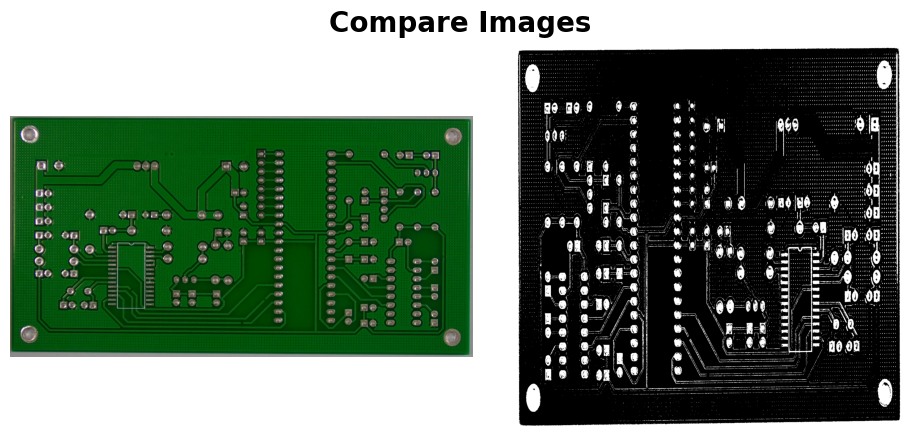
\includegraphics[width=0.8\textwidth]{preprocessing_results.png}
	\caption{Preprocessing Results of the Image Preprocessing Pipeline}
	\label{fig:preprocessing_results}
\end{figure}

\subsection{Overview of Implemented Preprocessing Operations}
A summary of the currently implemented preprocessing operations, categorized by their types, is provided in the following table:

\begin{longtable}{|p{0.3\linewidth}|p{0.65\linewidth}|}
	\hline
	\textbf{Category}                     & \textbf{Preprocessing Steps}                                                                                                                         \\
	\hline
	\endhead
	\hline
	\endfoot

	\textbf{Histogram Equalization}       & Adaptive Histogram Equalizer, Global Histogram Equalizer                                                                                             \\
	\hline
	\textbf{Blurring \& Smoothing}        & Gaussian Blur Filter, Median Blur Filter, Bilateral Filter, Average Blur Filter                                                                      \\
	\hline
	\textbf{Thresholding}                 & Otsu Thresholding, Adaptive Thresholding, Binary Thresholding, Truncated Thresholding, Threshold to Zero                                             \\
	\hline
	\textbf{Noise Reduction \& Injection} & Non Local Mean Denoiser, Gaussian Noise Injector                                                                                                     \\
	\hline
	\textbf{Color Space Conversion}       & RGB To Grayscale, Grayscale To RGB                                                                                                                   \\
	\hline
	\textbf{Geometric Transformations}    & Rotator, Mirrorer, Shape Resizer, Square Shape Padder                                                                                                \\
	\hline
	\textbf{Morphological Operations}     & Erosion Filter, Dilation Filter, Dilate Erode Sequencer                                                                                              \\
	\hline
	\textbf{Normalization}                & Min Max Normalizer, Standard Normalizer, Mean Normalizer, Local Contrast Normalizer                                                                  \\
	\hline
	\textbf{Random Augmentations}         & Random Color Jitterer, Random Sharpening, Random Rotator, Random Flipper, Random Cropper, Random Perspective Transformer, Random Elastic Transformer \\
	\hline
	\textbf{Miscellaneous}                & TypeCaster, Clipper, Scaler                                                                                                                          \\
	\hline
\end{longtable}

\subsection{Randomization of the Preprocessing Pipeline}
The framework offers a method to randomize the configurations of the preprocessing pipeline, which is useful for exploring the effects of different preprocessing settings on image datasets. This functionality is beneficial for hyperparameter optimization and various experimental scenarios. Users can specify ranges or distributions for each parameter within the JSON configuration, and the framework will randomly sample from these options during the application of the pipeline.


\section{Discussion}
The image preprocessing framework is specifically tailored to work with TensorFlow's image dataset format. This limitation results from the decision to manage the pipeline's processing by using TensorFlow's computational efficiencies. Despite this limitation, the integration of TensorFlow and OpenCV in the framework design provides an environment that is easy to use, modular, and extensible, supporting a broad range of preprocessing operations.

It is important to note that the framework does not include capabilities for learning or optimizing the parameters of preprocessing steps automatically. Instead, it focuses solely on preprocessing tasks to prepare data for subsequent model training, without involving model training itself. This separation ensures that the framework remains streamlined and efficient for its designated preprocessing functions.

Moreover, the framework's architecture is developed to emphasize simplicity, reproducibility, and modularity. These characteristics ensure that users can easily experiment with different preprocessing configurations and seamlessly integrate the framework into diverse machine learning environments. One of the significant features of the framework is its support for the randomization of pipeline configurations, which greatly assists in hyperparameter optimization. This feature increases the flexibility of the framework, allowing users to effectively explore and optimize preprocessing steps to suit specific requirements.

Overall, the framework provides a robust solution for managing image preprocessing pipelines, taking advantage of the capabilities of the TensorFlow ecosystem and OpenCV. Its design also accommodates the straightforward addition of new preprocessing operations, allowing for continuous improvement and adaptation to new challenges and advancements in the field of image processing.



% \section*{Acknowledgments}
% Good Acknowledgments here.

\bibliography{sample}

\end{document}
